% Expository adaptation, October 7, 2026. Original mathematics: OpenAI, September 23, 2026.
% Prose revised and explanations expanded; see README.md for the source and scope.
\section{Compile a supplied machine into a deterministic simulation}
\label{sec:compiler}

The approximation theorem begins by fixing a randomized machine. There is a separate uniformity question: can one algorithm take a machine description and its supplied resource bounds, and output a deterministic simulator together with explicit bounds for that simulator? This appendix gives that compiler.

The supplied time, space, and error bounds are hypotheses about the source. The compiler does not decide whether they are true. Instead, it uses one fixed resource-capped interpreter and one fixed deterministic approximator for that interpreter. Source-dependent padding puts every promised source computation within the interpreter's caps.

\begin{theorem}[Effective simulation with explicit bounds]
\label{thm:effective-simulation}
There is a terminating algorithm which, given a finite randomized machine
description $M$ and positive integers $a,b$, emits a deterministic
machine $D_M$ and positive integers $K,H,c$ with the following guarantee.
If, on every input of length $n$ and every random tape, $M$ halts within
$(n+2)^a$ steps, uses at most $b\lceil\log(n+2)\rceil$ work bits, and
has acceptance probability at most $1/3$ on no inputs and at least
$2/3$ on yes inputs, then $D_M$ decides the same language. On each input,
that same execution uses at most $K\log(n+2)$ work bits and
$H(n+2)^c$ elementary bit operations.
\end{theorem}

The compiler's own running time need only be finite, and its output
exponent may depend on the source.

The proof has four steps. Construct a single interpreter with unconditional resource bounds on every encoded input. Apply the approximation theorem to it once. Encode any promised source run as a sufficiently padded input to that fixed approximation program. Finally, generate the virtual-input routines and derive explicit bounds from their finite descriptions.

We prove Theorem~\ref{thm:effective-simulation} by specializing one fixed deterministic program. First we construct a randomized interpreter
$U$ that enforces polynomial-time and logarithmic-space bounds on every
input. Theorem~\ref{thm:fixed-precision} supplies a deterministic machine
$A$ that separates the inputs on which $U$ accepts with probability at
least $2/3$ from those on which it accepts with probability at most
$1/3$. Both $U$ and $A$ are fixed before the compiler receives a source
description $M$ and bounds $a,b$.

When the source satisfies its supplied resource bounds, padding places
each encoded computation within $U$'s caps without changing its
acceptance probability. The generated machine runs $A$ on that padded input, generating each requested
symbol from the real input. We then compute the output bounds $K,H,c$
from the generated finite transition table and the fixed library data.
The compiler never has to select a new probability approximator or infer
resource bounds from the source's behavior.

Universal deterministic estimation has a substantial antecedent in
Pyne, Raz and Zhan~\cite[full version, Theorem~5.1]{PyneRazZhan2023}.
They construct one deterministic algorithm that, on input $(1^n,\mathcal B)$
with $n\ge1$ and $\mathcal B$ an ordered branching program of length
and width at most $n$, approximates its acceptance probability to error less than
$1/n$. For every space-constructible $S(n)\ge\log n$, this single
algorithm uses $O(S(n))$ space exactly when
$\mathsf{prBPL}\subseteq\mathsf{SPACE}[O(S(n))]$.
Here the preceding sections establish the separator used by one fixed
library, and we compute explicit resource bounds for its source-specific
specialization.

All quantities in this section are local to the compiler construction.
In particular, $P$ is a padding exponent, $d_{\mathrm{code}}$ is a program
length, $B_n=\lceil\log_2(n+2)\rceil$, and $N_{\mathrm{pad}}$ is a virtual
input length.  They do not denote the statistical budgets, field modulus,
or domain sizes used in the preceding sections.  We use the usual
counted-cell convention for work tapes: traversed writable cells count
toward space, whether or not they contain a nonblank symbol.  The finite
control and the read-only input have their standard treatment.

\subsection{An interpreter that enforces its own resource limits}
\label{subsec:compiler-interpreter}

The interpreter must be small-space even on malformed or maliciously large descriptions. It therefore measures the whole input first, checks the code length before allocating storage, and imposes explicit time and tape limits during simulation. The coding below makes those checks finite scans of listed data.

Fix a binary coding of ordinary finite transition lists.  One concrete
choice uses a fixed record grammar and the field encoding
$w\mapsto 1^{|w|}0w$.  Lists specify the finite state set, tape and
alphabet declarations, initial and halting states, blanks and endmarkers,
and transition records.  A transition record lists its tested state,
scanned symbols and coin pattern, followed by its next state, written
symbols and local head movements.  The grammar has fixed nesting depth;
its fields are actual listed data, not recursively executable descriptions.
State and symbol IDs are canonical binary integers used only as names.
The first matching transition is
used; a missing transition causes rejection.  Wildcards for ignored coins
can equivalently be expanded into a finite explicit list.

Write $z$ for a program in this coding and
$d_{\mathrm{code}}=|z|\ge1$.  The coding permits at most
$d_{\mathrm{code}}$ work tapes and a block of at most
$d_{\mathrm{code}}$ fresh fair bits per simulated transition.  Every ID
has at most $d_{\mathrm{code}}$ bits.  A harmless padding field can enlarge
the program to meet these inequalities.  All tape movements are local.
Work coordinates are measured from their initial origins; the ordinary
model has one input head and one head per work tape.  For a source input
$x$ of length $n$, let $E_{d_{\mathrm{code}}}(x)$ encode each of its
symbols by its ID padded to exactly $d_{\mathrm{code}}$ bits.

\paragraph{Preserving the supplied source bounds.}
An ordinary source machine $M$ can be converted effectively to this format
by renaming its states and symbols and listing its transitions.  Its tapes
are represented directly, so a source transition retains its work writes
and head movements and counts as one interpreted transition.  The
conversion does not pass through a slower single-tape simulation.

Under the optional one-way read-only random-tape convention, the source
may reuse its current random bit. Store a cached bit and a validity flag
in finite control, initially invalid.
At each transition obtain one fresh bit.  Use it if the cache is invalid;
otherwise use the cached bit and discard the fresh one.  Execute the
source transition, then retain the used bit if the random head stayed
and invalidate the cache if it advanced.  This samples a newly visited
random cell lazily on its next use.  It preserves the joint distribution
of the source run and needs no initialization transition.  An initially
halting state is recognized before the first transition.  The same
argument uses a fixed finite block for a convention allowing finitely
many fresh bits per elementary transition, discarding unused bits.
The finite cache changes neither counted work space nor the number of
source transitions.  Thus the supplied parameters $a,b$ remain valid;
only the static description length can increase.

\begin{lemma}[A total resource-capped interpreter]
\label{lem:compiler-interpreter}
There is one fixed randomized Turing machine $U$ with polynomial
worst-case running time and $O(\log(m+2))$ counted work bits on every
binary input of length $m$, with the following behavior.
Set
\begin{equation}\label{eq:compiler-interpreter-cap}
 \lambda_m=\lceil\log_2(m+2)\rceil,
 \qquad
 R(m,d_{\mathrm{code}})
   =\left\lfloor\frac{\lambda_m}
       {100(d_{\mathrm{code}}+1)^3}\right\rfloor.
\end{equation}
On an input with prefix
\begin{equation}\label{eq:compiler-prefix}
  1^{d_{\mathrm{code}}}0\,z\,1^n0\,
  E_{d_{\mathrm{code}}}(x),
\end{equation}
it first requires $1\le d_{\mathrm{code}}\le\lambda_m$ and
$R(m,d_{\mathrm{code}})\ge1$.  It then simulates the encoded machine
for at most $m$ transitions, allowing each counted work tape only
coordinates in $[-R,R]$.  It rejects malformed data, a requested move
outside these bounds, or failure to halt by the end of the transition
budget.  Otherwise it returns the encoded machine's decision.  The
suffix after the complete prefix has no parsing significance.
\end{lemma}

\begin{proof}
First validate the input before allocating any description-dependent storage. Count $m$ before interpreting the prefix.  Scan the unary code-length
header with a bounded counter, rejecting if its length exceeds
$\lambda_m$ or the required delimiter is absent.  Check the two
eligibility conditions before copying $z$ or allocating simulation
storage.  Then verify that the following $d_{\mathrm{code}}$ code bits,
the unary data-length header, and the required data bits are present.
The parsed $n$ is at most $m$, and
$d_{\mathrm{code}}n\le\lambda_m m$, so even size calculations preceding
a failed length check use only $O(\lambda_m)$ bits.  List counts, ID
lengths, tape declarations, and movements are checked against the actual
code and the stated bounds before any loops or allocations using them.
There is no enumeration of an implicit domain of symbol or state names.

The eligibility conditions now imply a simultaneous storage bound for all encoded tapes and administrative records. Store the encoded tapes sequentially on a fixed number of real work
tapes of $U$.  At most $d_{\mathrm{code}}$ strips, each with $2R+1$
cells of $d_{\mathrm{code}}$ bits, require
\begin{equation}\label{eq:compiler-interpreter-space}
 d_{\mathrm{code}}^2(2R+1)=O(\lambda_m)
\end{equation}
bits.  Indeed, eligibility gives
$d_{\mathrm{code}}^3\le\lambda_m$ and
$d_{\mathrm{code}}^2R\le\lambda_m$.
The copied program, current state, scanned and written symbol tuples,
coin block, strip coordinates, step counter, and parsing scratch fit
simultaneously in $O(\lambda_m)$ bits.  A single simulated input-head
coordinate has magnitude $O(m)$ by the transition cap and therefore
also uses $O(\lambda_m)$ bits.  Read the corresponding source symbol
by rescanning the encoded data, supplying the appropriate markers or
off-data blanks according to the encoded input-tape convention.

All routines are bounded scans and ordinary binary arithmetic.  They
iterate over actual code positions, input positions, a bounded tape/head
list, strip positions, and bit positions, with a fixed nesting depth.
Each range is polynomially bounded in $m+2$; binary arithmetic is
implemented by bit scans, not unit-cost operations on growing words.
Matching a listed transition, fetching input symbols, updating the
strips, and obtaining its finite coin block therefore take polynomial
time in $m+2$, with one fixed exponent determined by these routines.
The same bounds hold when a check fails.  There are at most $m$
interpreted transitions.  Checking the initial halting state and the
state reached by the last permitted transition gives the asserted
total behavior, including $m=0$.  The resulting fixed $U$ has the
required polynomial worst-case time on every random tape.
\end{proof}

No bounded-error language promise is asserted for $U$ on arbitrary
inputs.  Its acceptance probability may lie between $1/3$ and $2/3$.
This is why we use probability approximation rather than a bare
language-class containment.

\subsection{Fix the deterministic approximator once}
\label{subsec:compiler-library}

The interpreter need not itself decide a bounded-error language on arbitrary encodings. This causes no difficulty because our theorem approximates arbitrary acceptance probabilities. Apply Theorem~\ref{thm:fixed-precision} to the fixed machine $U$ and
accuracy exponent $3$, and compare its dyadic answer with $1/2$.
The error on an input of length $m$ is at most
$(m+2)^{-3}\le1/8$.  Hence the resulting deterministic machine accepts
whenever $\Pr[U\text{ accepts}]\ge2/3$ and rejects whenever that
probability is at most $1/3$, since
\[
 \frac13+\frac18=\frac{11}{24}<\frac12
   <\frac{13}{24}=\frac23-\frac18.
\]
It halts on every input, including inputs between the two thresholds,
as also stated in Corollary~\ref{cor:promise-bpl}.  Its logarithmic
space bound counts all simultaneously live work in the approximation
algorithm.  Store the $O(\log(m+2))$-bit dyadic output in work space
for the threshold test.

We fix this library once in the following convenient form.  It is an
ordinary finite-tape deterministic decision machine $A$ with one input
head confined to the endmarked input, initially at its left endmarker,
such that every work head stays in
\begin{equation}\label{eq:compiler-library-box}
 [-(\lambda_m+1),\lambda_m+1]
\end{equation}
relative to its origin.  To obtain this form, first consolidate any
input heads by keeping their coordinates in logarithmic work space
and scanning for each read.  Even an off-data coordinate under an
unbounded-input convention has logarithmic length because the original
library has polynomial running time.  A fixed change of initial control
state handles its input-head start convention.

Next choose an integer $w$ at least a coefficient bounding each counted
work head's distance from its origin by $w\lambda_m$.  Such one fixed
$w$ exists from the logarithmic bound, enlarged if necessary for the
finitely many small lengths.  Group consecutive work cells into blocks
of width $w$, storing within-block offsets in finite control.  The
resulting finite alphabet and finite transition list realize
Equation~\eqref{eq:compiler-library-box}, also for two-sided tapes.
All symbol widths will be charged in bits below; grouping only exposes
a uniform address bound and gives no uncharged bit compression.

This choice of $A$, including its one blocking width, precedes every
compiler input.  More formally, the remaining construction is a
computable syntactic function of a finite library list and
$(M,a,b)$.  Fixing one valid finite list yields one ordinary
computable compiler on all those source inputs.  It does not require
an algorithm that discovers a separator or a logarithmic-space
coefficient from an arbitrary machine description.  The existence
of the fixed list was proved by Theorem~\ref{thm:fixed-precision};
no constant is selected as a noncomputable function of the source
machine or its ordinary input.

The fixed finite data are the program grammar, the transition list of
$A$ with its blocked work alphabets and head conventions, and the
finite callback templates described below. The construction constants,
cutoffs, generator choices and finite instruction routines used by the
separator are included in that list. Its blocking width is fixed at
the same time. These are data specifying one compiler; subsequent
source-dependent integers are computed from these data and the supplied
$(M,a,b)$.

\subsection{Use padding to fit the promised source computation}
\label{subsec:compiler-padding}

The deterministic approximator is now fixed, independently of the source description. We enlarge its virtual input enough that the interpreter's work strips and transition limit contain every promised source run. No branch of such a run is cut off, so acceptance probability is preserved exactly.

Given the source description and its supplied positive integers $a,b$, construct $z$ as above and compute
\begin{equation}\label{eq:compiler-padding}
 \begin{split}
 P&=1000(d_{\mathrm{code}}+2)^4(a+b+2),\\
 B_n&=\lceil\log_2(n+2)\rceil,
 \qquad N_{\mathrm{pad}}=2^{PB_n}.
 \end{split}
\end{equation}
The generated machine will run $A$ on a virtual binary input
$y_x$ of length $N_{\mathrm{pad}}$ whose prefix is
Equation~\eqref{eq:compiler-prefix} and whose remaining bits are zero.
Its prefix length is exactly
\begin{equation}\label{eq:compiler-prefix-length}
 L_{\mathrm{pre}}
 =(d_{\mathrm{code}}+1)+d_{\mathrm{code}}+(n+1)
       +d_{\mathrm{code}}n
 =(d_{\mathrm{code}}+1)(n+2).
\end{equation}
Since $B_n\ge1$, $2^{B_n}\ge n+2$, and
$2^{P-1}\ge d_{\mathrm{code}}+1$, this length is at most
$N_{\mathrm{pad}}$.  The interpreter's length parameter is
\begin{equation}\label{eq:compiler-padded-log}
 \ell_{\mathrm{pad}}
 :=\lambda_{N_{\mathrm{pad}}}=PB_n+1.
\end{equation}

All eligibility checks pass.  In particular,
\[
 \frac{P}{100(d_{\mathrm{code}}+1)^3}
 =10\frac{(d_{\mathrm{code}}+2)^4}
          {(d_{\mathrm{code}}+1)^3}(a+b+2)
 \ge30(a+b+2),
\]
so
\begin{equation}\label{eq:compiler-strip-slack}
 R(N_{\mathrm{pad}},d_{\mathrm{code}})
 \ge30(a+b+2)B_n-1\ge(a+b)B_n+4.
\end{equation}
Also $P>a$, whence
$(n+2)^a\le2^{aB_n}<N_{\mathrm{pad}}$.
Local motion from an initial work origin to a cell entails visiting
the intervening counted cells.  The source bound of $bB_n$ work bits
therefore places every source work cell in the allocated strip;
the slack in Equation~\eqref{eq:compiler-strip-slack} also covers a final
one-cell move.  This uses the source's original cell costs, each at
least one bit, and does not charge it for the larger interpreter IDs.

Consequently no resource cutoff changes a promised source run, and
\begin{equation}\label{eq:compiler-exact-probability}
 \Pr[U(y_x)\text{ accepts}]=\Pr[M(x)\text{ accepts}].
\end{equation}
There is no conditioning or additional approximation in this equality.
The decision of $A(y_x)$ is therefore the decision required for $L_M$.
Although $N_{\mathrm{pad}}$ is given exponentially, it is at most
$(n+2)^{2P}$ for the fixed source.  More importantly, it need never
be written as an input string.

\begin{remark}[Optional head conventions]
The construction also applies when the fixed coding and $U$ are chosen
to allow at most $d_{\mathrm{code}}$ heads per tape, with the usual common
initial origin. These conventions are fixed before choosing $A$.
There are then at most $d_{\mathrm{code}}^2$ work-head coordinates and
scanned symbols.  Their storage is bounded by
\[
 O\bigl(d_{\mathrm{code}}^2\log(2R+1)
          +d_{\mathrm{code}}^3\bigr)=O(\lambda_m).
\]
For multiple input heads, or an optional entirely blank tape whose
cells are not charged, use signed $R$-bit coordinates and reject on
overflow.  At most $d_{\mathrm{code}}^2$ such coordinates still cost
$O(d_{\mathrm{code}}^2R)$ bits.  These optional conventions do not
change the interpreter's bounds. The padded instances just constructed
never overflow those coordinates.

Under the optional head conventions, local motion bounds an input or
uncharged blank-tape coordinate by the source time, up to the fixed
endmarker offset.  Its signed encoding fits because $R\ge aB_n+4$.
\end{remark}

Figure~\ref{fig:compiler-padding} shows how the generated machine supplies
the virtual input requested by $A$. The library's work tapes remain live
while the callback scans the real input; the resource bound below counts
the library and callback storage simultaneously.

\begin{figure}[tb]
 \centering
 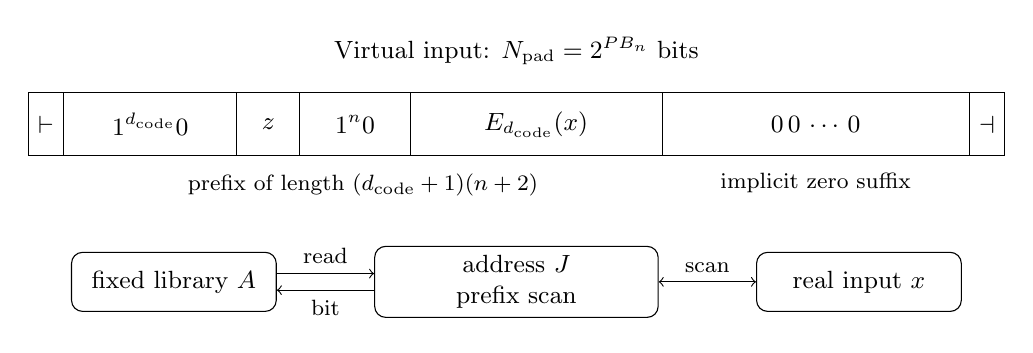
\begin{tikzpicture}[x=1cm,y=1cm,font=\small]
  \draw (0,0) rectangle (12.4,0.8);
  \draw (0.45,0) -- (0.45,0.8);
  \draw (2.65,0) -- (2.65,0.8);
  \draw (3.45,0) -- (3.45,0.8);
  \draw (4.85,0) -- (4.85,0.8);
  \draw (8.05,0) -- (8.05,0.8);
  \draw (11.95,0) -- (11.95,0.8);
  \node at (0.225,0.4) {$\vdash$};
  \node at (1.55,0.4) {$1^{d_{\mathrm{code}}}0$};
  \node at (3.05,0.4) {$z$};
  \node at (4.15,0.4) {$1^n0$};
  \node at (6.45,0.4) {$E_{d_{\mathrm{code}}}(x)$};
  \node at (10,0.4) {$0\,0\,\cdots\,0$};
  \node at (12.175,0.4) {$\dashv$};
  \node[anchor=south] at (6.2,1.03)
    {Virtual input: $N_{\mathrm{pad}}=2^{PB_n}$ bits};
  \node[anchor=north,font=\footnotesize] at (4.25,-0.1)
    {prefix of length $(d_{\mathrm{code}}+1)(n+2)$};
  \node[anchor=north,font=\footnotesize] at (10,-0.1)
    {implicit zero suffix};
  \node[draw,rounded corners,align=center,minimum width=2.6cm,
        minimum height=0.75cm] (library) at (1.85,-1.6)
    {fixed library $A$};
  \node[draw,rounded corners,align=center,minimum width=3.6cm,
        minimum height=0.75cm] (callback) at (6.2,-1.6)
    {address $J$\\prefix scan};
  \node[draw,rounded corners,align=center,minimum width=2.6cm,
        minimum height=0.75cm] (realinput) at (10.55,-1.6)
    {real input $x$};
  \draw[->] ([yshift=3pt]library.east) -- ([yshift=3pt]callback.west)
    node[midway,above,font=\footnotesize] {read};
  \draw[->] ([yshift=-3pt]callback.west) -- ([yshift=-3pt]library.east)
    node[midway,below,font=\footnotesize] {bit};
  \draw[<->] (callback.east) -- (realinput.west)
    node[midway,above,font=\footnotesize] {scan};
\end{tikzpicture}


 \caption{The fixed library reads the padded input through a callback.
 The callback regenerates prefix symbols from the real input and returns
 zero for an address in the padding interval.}
 \label{fig:compiler-padding}
\end{figure}

\subsection{Read the padded input without storing it}
\label{subsec:compiler-callback}

The padded string can be much longer than the real input. Only its current queried address needs to be stored. A finite routine answers that query by scanning the short encoded prefix and returning zero if the address lies in the padding. We now give the routine explicitly so that its memory is counted alongside the suspended approximator.

Inline the finite transition list of $A$, giving it its own work tapes.
The generated machine $D$ suspends its library control state in finite
control during an input operation.  Four auxiliary binary words suffice:
the length count $n+1$, the virtual right-endmarker address
$N_{\mathrm{pad}}+1$, the virtual input-head position $J$, and a prefix
position $I$.  Each has a separate tape, with origin and termination
marks and digits in low-end-first order.

Initialize the length count to one and increment it once per real input
symbol.  Its bit length is exactly
\begin{equation}\label{eq:compiler-bitlength}
 \operatorname{bitlength}(n+1)
   =\lfloor\log_2(n+1)\rfloor+1
   =\lceil\log_2(n+2)\rceil=B_n
 \qquad(n\ge0).
\end{equation}
For every bit place in that count, write $P$ zero bits on the bound tape,
then append a one.  This produces the low-end-first representation of
$2^{PB_n}=N_{\mathrm{pad}}$; increment it to obtain
$N_{\mathrm{pad}}+1$.  The repetition of $P$ is hardwired finite control.
Initially set $J=0$, the library's left-endmarker position.

At a virtual read, first test $J=0$ and $J=N_{\mathrm{pad}}+1$ and return
the corresponding endmarker.  Otherwise initialize $I=1$ and regenerate
the prefix in its natural order:
\begin{enumerate}
 \item emit the fixed string $1^{d_{\mathrm{code}}}0z$;
 \item scan $x$, emitting one $1$ per symbol, and then emit $0$;
 \item rewind and scan $x$ again, emitting each fixed-width symbol code
       in $E_{d_{\mathrm{code}}}(x)$.
\end{enumerate}
Here ``emit'' means compare the current $I$ with $J$, return the bit
if they agree, and otherwise increment $I$ and continue.  If the scan
finishes without a match, return zero.  The strings $z$, the integer
$d_{\mathrm{code}}$, symbol codes and emission phases are fixed in
the generated control.  The real input head is rewound by scanning to
its endmarker, without storing its position.  In particular,
$J=N_{\mathrm{pad}}+1$ is answered before regeneration, while a padding
address such as $J=N_{\mathrm{pad}}$ returns zero after the finite
prefix scan.  The largest prefix counter value is
$L_{\mathrm{pre}}+1\le N_{\mathrm{pad}}+1$.

For explicit counter routines, an increment uses a finite carry flag.
Compare two low-end-first words by scanning both, retaining only a
finite comparison flag that is overwritten by each higher differing
bit.  After one terminator, treat its later bits as zero using a finite
``ended'' flag.  Rewind each tape to its origin mark afterward.  Zeroing
and copying are likewise bounded bit scans.  No growing arithmetic
register beyond the named words is required.  All words have at most
$PB_n+2$ bits; including delimiters and rewinds, their heads need visit
only positions through $PB_n+10$.

After the callback, perform the indicated library transition and update
$J$ in place for its input-head motion.  The library's work heads and
contents are untouched by the callback.  Its state, the returned input
symbol, and any step-local scanned tuple are fixed finite-control data.
The callback does not invoke $A$ recursively or maintain a stack of
callbacks.  The real input head stays between its real endmarkers.

Every listed routine terminates.  For example, a complete regeneration
uses at most $L_{\mathrm{pre}}$ emissions, each with an
$O(PB_n+1)$-bit comparison and increment, together with two real-input
scans.  Initialization makes $n$ increments and writes $PB_n+1$ bound
bits.  These observations give direct polynomial bounds for the
auxiliary operations.  The whole simulation halts because $A$ is total.
Its more uniform explicit time bound, including every such operation,
is derived next from the complete configurations of this same machine.

All the above instructions can be generated as finite transition tables,
unrolling fixed repetitions and strings if necessary.  Formation of the
source list, the integer $P$, and this transition table is a finite
effective process.  It makes no test of the source's semantic error or
resource promises.  Syntactically invalid compiler inputs may be assigned
a fixed default output; correctness is required on the stipulated class.
The generated simulation is total and obeys the bounds below even when
the supplied source promises fail; those promises are used to establish
that its decision agrees with the source.

\subsection{Compute explicit bounds for the generated machine}
\label{subsec:compiler-bounds}

All source-dependent choices have now been made by finite operations on code and supplied integers. The remaining bounds use three concrete counts: work tapes, alphabet sizes, and control states. We first bound all live work bits, then count complete configurations of the halting machine, and finally convert finite-alphabet transitions to elementary bit operations.

Use the finite-alphabet description just constructed to compute $t$, its
number of work tapes; $g\ge2$, the maximum of two and its work alphabet
sizes, including all blank, origin and termination symbols; and $q_D$,
its number of states, including callback phases.  Let $u\ge1$ dominate
its explicit transition-table bit length, all alphabet sizes (including
the input alphabet), the number of states, and the number of tapes.
Padding this integer is effective.  Return the positive integer bounds
\begin{equation}\label{eq:compiler-output-bounds}
 \begin{split}
 \rho&=100(P+2),\qquad
 S=1+(t+1)(2\rho+1)(g+2),\\
 K&=4S,\qquad c=2S+1,\qquad
 H=2^{(u+100)^2}(q_D+1).
 \end{split}
\end{equation}
These depend on the fixed source and the fixed library, and are computed
from finite syntax.  They have no dependence on $n$ or $x$.

\paragraph{All live work bits.}
Every work head stays in
$[-\rho B_n,\rho B_n]$.  For a library tape this follows from
Equations~\eqref{eq:compiler-library-box} and
\eqref{eq:compiler-padded-log}, since
$\ell_{\mathrm{pad}}+1=PB_n+2\le\rho B_n$.
For an auxiliary tape it follows from
$PB_n+10\le\rho B_n$, using $B_n\ge1$.
Thus the library's live data and all callback data satisfy the same
bound at the same time.  Encoding a work alphabet of size $g_i$ in
$\max\{1,\lceil\log_2 g_i\rceil\}\le g$ bits per symbol bounds
their total data by
\begin{equation}\label{eq:compiler-space-bound}
 t(2\rho B_n+1)g\le SB_n.
\end{equation}
Even twice this quantity satisfies the stronger logarithmic bound: with
$L_n=\log_2(n+2)\ge1$ we have $B_n\le2L_n$ and
\[
 2SB_n\le4SL_n=K L_n.
\]

\paragraph{All finite-alphabet transitions.}
For a fixed real input $x$, a complete configuration is specified by
the state, the real input-head position, all work-head positions, and
all work symbols in the stated intervals.  Everything outside these
intervals remains at its initial value.  There are at most
\begin{equation}\label{eq:compiler-configurations}
 q_D(n+2)(2\rho B_n+1)^t
       g^{t(2\rho B_n+1)}
 \le q_D(n+2)2^{SB_n}
 \le q_D(n+2)^c
\end{equation}
such configurations.  For the first inequality use
\[
 2\rho B_n+1\le(2\rho+1)B_n,
 \quad \log_2g\le g,
 \quad \log_2(2\rho B_n+1)\le(2\rho+1)B_n;
\]
the second uses $B_n\le2\log_2(n+2)$ and $c=2S+1$.
A deterministic halting computation cannot repeat a complete
configuration.  Therefore Equation~\eqref{eq:compiler-configurations}
bounds its total transitions, including initialization, counter
arithmetic, every regenerated input bit, and every library transition.
The virtual head position is already in the counted word $J$; it is
not an additional uncounted configuration component.

\paragraph{Elementary bit operations.}
The preceding count refers to ordinary finite-alphabet transitions.
To charge them in bits, encode each work symbol by a fixed-width block,
mapping blank to the all-zero block.  Read and write within the current
block, return to its first bit, and move to the first bit of the target
block.  Within-block phases and scanned finite tuples are stored in
finite control.  No per-block writable delimiter is needed, and these
operations visit only blocks whose macro positions occur in the proved
work intervals.  Existing origin and termination symbols have already
been included in $g$.  Thus the block implementation obeys the bit-space
estimate above; the factor two also allows the usual blank/bit tape
convention.  Input-symbol access has fixed width and is covered by the
same finite description parameter $u$.

There are at most $u+1$ scanned symbols of at most $u$ bits each.
An explicit sequential comparison against at most $u$ transition rows,
followed by the fixed-width reads, writes and moves, uses at most a
fixed polynomial in $u+1$ bit actions per transition.  For example,
the deliberately loose bound $100(u+1)^8$ suffices for these scans
and comparisons, with all temporary phase and symbol information in
finite control.  It is dominated, for $u\ge1$, by
\[
 100(u+1)^8\le2^{(u+100)^2}.
\]
The binary microcode may have more states than $q_D$, but no new
configuration count is needed: multiply the number of original
transitions by this per-transition bit cost.  Equations~\eqref{eq:compiler-output-bounds}
and~\eqref{eq:compiler-configurations} give the simultaneous bound
\begin{equation}\label{eq:compiler-time-bound}
 \operatorname{time}_{\mathrm{bit}}(D,x)
 \le H(n+2)^c.
\end{equation}
No growing-word arithmetic is charged as a single elementary bit action.

\begin{proof}[Completion of the proof of Theorem~\ref{thm:effective-simulation}]
The compiler returns the described machine $D$ and the integers
$K,H,c$ in Equation~\eqref{eq:compiler-output-bounds}.  Its finite
syntactic construction terminates.  On every promised source input,
Equation~\eqref{eq:compiler-exact-probability} and the fixed separator's
threshold guarantee give the correct decision.  The totality of $A$
and the finite callback loops prove halting.  Equations~\eqref{eq:compiler-space-bound}
and~\eqref{eq:compiler-time-bound} give at most $K\log_2(n+2)$
work bits and $H(n+2)^c$ bit operations for this same machine.

All claims include $n=0$: then $B_n=1$, the real-input scans are empty,
the count $n+1=1$ has one bit, and every displayed padding, strip,
space, and time inequality remains valid.  The library's grouping
width already includes its finitely many small-length exceptions.
All construction constants are fixed before the ordinary input is read.

The work and time internal to probability approximation---environment
enumeration, numerical digits, recursive interfaces, recomputation,
and precision management---belong to the one complete library machine
proved in Theorem~\ref{thm:fixed-precision}.  Its tapes remain counted
throughout virtualization.  The compiler adds only the exact input
operations analyzed here, without an evaluation oracle or an external
stack.  Configuration counting gives polynomial time because this
entire deterministic machine uses exact logarithmic space.
\end{proof}

